%% LyX 1.3 created this file.  For more info, see http://www.lyx.org/.
%% Do not edit unless you really know what you are doing.
\documentclass[english]{article}
\usepackage[T1]{fontenc}
\usepackage[latin1]{inputenc}
\usepackage{geometry}
\geometry{verbose,letterpaper,tmargin=1in,bmargin=1in,lmargin=1in,rmargin=1in,headheight=0.2in,headsep=0.25in,footskip=0.5in}
\usepackage{array}
\usepackage{varioref}
\usepackage{graphicx}

\makeatletter

%%%%%%%%%%%%%%%%%%%%%%%%%%%%%% LyX specific LaTeX commands.
%% Because html converters don't know tabularnewline
\providecommand{\tabularnewline}{\\}

%%%%%%%%%%%%%%%%%%%%%%%%%%%%%% Textclass specific LaTeX commands.
 \usepackage{verbatim}

\usepackage{babel}
\makeatother
\begin{document}

\title{Quantum GIS Design Document}


\author{QGIS Core Design Team%
\footnote{Gary E Sherman, Mark Coletti, Denis Antipov%
}}

\maketitle
\newpage
\tableofcontents{}
\newpage


\section{Introduction}

This document describes the requirements and design for Quantum GIS
(QGIS), a desktop GIS application for Linux and Unix. This document
presents use cases, high-level class diagrams, and additional information
about the design and implementation of QGIS. 

QGIS is hosted on SourceForge at http://qgis.sourceforge.net. The
current release of QGIS is a viewer with a minimal feature set, including
loading data, browsing, and identifying features.

The design outlined in this document represents the next phase of
QGIS development, which will move the application to a flexible and
extensible platform for working with spatial data.

Note that it's presumed that the reader is familiar with C++, object-oriented
design, and UML.


\section{Definitions}

The following is a list of definitions for terms used in this document.
Some of these definitions are taken from the Association for Geographic
Information and the University Of Edinburgh Department of Geography
online dictionary of GIS terms available at http://www.geo.ed.ac.uk/agidict/welcome.html.

\begin{description}
\item [Attribute:]A fact describing an entity in a relational data model,
equivalent to the column in a relational table.
\item [Feature:]A set of points, lines or polygons in a spatial database
that represent a real-world entity. The terms feature and object are
often used synonymously.
\item [GIS:]Geographic Information System. A software system that provides
the ability to view and analyze spatial data and its attributes.
\item [\label{des:Layer:-A-dataset}Layer:]A dataset that has a spatial
context and can be drawn on a map canvas. Layers may have associated
attributes. 
\item [Plugin:]A compiled library that can be dynamically loaded into an
application to provide new functionality.
\item [Projection:]A method of representing the earth's three-dimensional
surface as a flat two-dimensional surface. This normally involves
a mathematical model that transforms the locations of features on
the earth's surface to locations on a two-dimensional surface. Because
the earth is three-dimensional, some method must be used to depict
the map in two dimensions. Therefore such representations distort
some parameter of the earth's surface, be it distance, area, shape,
or direction.
\end{description}

\section{History}

The QGIS project was registered with SourceForge on June 15, 2002.
Since that time, QGIS has developed into a minimally functional viewer
with support for shapefiles%
\footnote{ESRI format for file-based spatial data.%
} and vector data stored in a PostgreSQL%
\footnote{PostgreSQL Relational Database - http://www.postgresql.org%
} database using the PostGIS%
\footnote{PostGIS extension - http://postgis.refractions.net%
} extensions.~

The development thus far has been useful in developing an understanding
of the challenges involved in developing a more robust Open Source
desktop GIS application. In March 2003, planning began to restructure
QGIS in order to make it more extensible and to provide a means to
add advanced functionality through the use of plugins.

The current version of QGIS (0.0.9) is still usable as a simple GIS
viewer for shapefiles and PostGIS layers. Only minor maintenance is
being done on the current code base at this time. 


\section{Goals}

There are already other Open Source GIS projects available today.
Many have asked what purpose QGIS will serve:

\begin{itemize}
\item Will QGIS be a complete desktop GIS application? 
\item Will it compete with commercial products?
\item Why are you developing another GIS application?
\end{itemize}
The answers to these questions are not clear-cut. A list of high-level
goals for the QGIS project are enumerated below. The reader can perhaps
use this information to answer these and other questions related to
the project:


\subsection{List of Goals}

\begin{enumerate}
\item Provide an easy to use desktop GIS application
\item Provide an easy to install application for users with minimum system
experience
\item Support common data formats
\item Provide the foundation for more advanced tools (plugins)
\item Become a tool for spatial data collection
\item Support data analysis and conversion
\item Print/plot maps
\item Integrate with Internet mapping technologies
\end{enumerate}
Section \ref{sec:Requirements} provides details about the functional
requirements.


\section{\label{sec:Requirements}Requirements}

This section describes the functional requirements of Quantum GIS.
These functional requirements drive the use cases discussed in Section
\ref{sec:Use-Cases}.

QGIS will provide GIS functionality somewhere between a simple viewer
and an industrial strength application. The ultimate nature of QGIS
is only limited by the talent of those software engineers who will
provide advanced capabilities through plugins.

Some of the major design requirements include:

\begin{itemize}
\item Extensible architecture using plugins
\item Internationalization
\item Integrated scripting language
\item Projection on-the-fly
\item Flexible symbology for all feature classes
\item Ability to render and browse data in many formats:

\begin{itemize}
\item Spatio-temporal data using a feature-centric model
\item Shapefiles
\item PostgreSQL / PostGIS layers
\item Raster
\end{itemize}
\item Support for OpenGIS implementation Specifications

\begin{itemize}
\item Geography Markup Language (GML)
\item Web Feature Service (WFS) 
\end{itemize}
\end{itemize}

\subsection{User Interface}

QGIS will use the SDI (Single Document Interface). QGIS currently
has (and will have) standard GUI interface elements such as menus,
toolbar, and a statusbar. In addition, the standard QGIS interface
will have a legend panel and a map canvas (or drawing area).


\subsection{Standards}

Development of QGIS will proceed with adoption of applicable OpenGIS
standards. This will include support for GML and possibly WFS.


\subsection{Data Formats}

Any data format could be supported by the development of a plugin
that reads and renders the data store. The {}``standard'' formats
that will be included in the core QGIS are similar to those currently
supported:

\begin{itemize}
\item Shapefiles
\item PostgreSQL/PostGIS
\item Rasters
\end{itemize}
Format support will be provided by plugins.


\subsection{Platform Support}

Initially, QGIS will target Linux and other Unix operating systems
supported by the Qt toolkit. Coding during development of QGIS and
plugins will be done in a way so as to not introduce any platform
dependencies. This will provide to possibility of a Windows version
at some point in the future. 


\subsection{Toolkits}

QGIS will leverage existing libraries and toolkits to support the
GUI, GIS data stores, and GIS processing algorithims. At present the
identified toolkits include:

\begin{itemize}
\item Qt (http://www.trolltech.com)
\item GDAL and OGR (/http://www.remotesensing.org/gdal)
\item Proj.4 (http://www.remotesensing.org/proj/)
\end{itemize}

\section{\label{sec:Use-Cases}Use Cases}

Use cases provide a means to identify and visualize the major goal
oriented tasks the application should address. 


\subsection{Actors}

Actors are really persons (or physical entities) that use a system
to acheive a specific goal (these goals are expressed as use cases).
A number of actors could be defined for QGIS, however at this point
the simple approach is taken. The actors are:

\begin{itemize}
\item Casual GIS User
\item Professional GIS User
\end{itemize}
These two actors are sufficient to frame the development and discussion
of QGIS use cases.


\subsection{Primary Use Cases}

The primary use cases for QGIS are listed below in no particular order
of importance:
\smallskip{}

\begin{tabular}{p{2.5in}p{2.5in}}
\begin{itemize}
\item Load data
\item Browse data
\item Install plugin
\item Find feature
\item dislayFeatureAttributes
\item Get help
\item Customize 
\item Save project
\item Restore project
\item Navigate map

\begin{itemize}
\item Pan
\item Zoom
\end{itemize}
\item Save image
\item Print

\begin{itemize}
\item Print image
\item Print metadata
\item Print feature information
\end{itemize}
\item Write script\end{itemize}
&
\begin{itemize}
\item Run script
\item Edit data

\begin{itemize}
\item Digitize
\end{itemize}
\item Buffer feature
\item Process data

\begin{itemize}
\item Union
\item Merge
\item Intersect
\end{itemize}
\item Convert data

\begin{itemize}
\item Change projection
\end{itemize}
\item Import data
\item Export data

\begin{itemize}
\item Export selected set
\end{itemize}
\item Select features

\begin{itemize}
\item Select by attribute
\item Select spatially
\end{itemize}
\item Edit Layer Preferences

\begin{itemize}
\item Edit Symbology
\item Edit Labels\end{itemize}
\end{itemize}
\tabularnewline
\end{tabular}


\subsection{Case Descriptions}

In the sections that follow, the use cases are presented in no particular
order.


\subsubsection{\label{sub:Load-Data}Load Data }

\begin{tabular}{p{2in}p{3in}}
\smallskip{}
\textbf{Use Case:}&
\smallskip{}
Load Data\tabularnewline
\smallskip{}
\textbf{Goal in Context:}&
\smallskip{}
Load a data set from a data set\tabularnewline
\smallskip{}
\textbf{Scope \& Level:}&
\smallskip{}
Primary task\tabularnewline
\smallskip{}
\textbf{Preconditions:}&
\smallskip{}
Application is running\tabularnewline
\smallskip{}
\textbf{Success End Condition:}&
\smallskip{}
Data is loaded and displayed\tabularnewline
\smallskip{}
\textbf{Failed End Condition:}&
\smallskip{}
Application is in pre-load state \tabularnewline
\smallskip{}
\textbf{Primary Actor(s):}&
\smallskip{}
Casual, Professional user\tabularnewline
\smallskip{}
\textbf{Trigger:}&
\smallskip{}
User wants to load data into environment for use\tabularnewline
\smallskip{}
\textbf{Description of Steps:}&
\begin{tabular}{|c|l|}
\hline 
User&
System\tabularnewline
\hline
\hline 
selects data&
\tabularnewline
\hline 
&
acknowledges\tabularnewline
\hline 
start load&
\tabularnewline
\hline 
&
system shows loading of data then shows data\tabularnewline
\hline
\end{tabular}\tabularnewline
\end{tabular}


\subsubsection{Browse Data}

\begin{tabular}{p{2in}p{3in}}
\smallskip{}
\textbf{Use Case:}&
\smallskip{}
Browse Data\tabularnewline
\smallskip{}
\textbf{Goal in Context:}&
\smallskip{}
Browse through a loaded data set and its features\tabularnewline
\smallskip{}
\textbf{Scope \& Level:}&
\smallskip{}
Primary task\tabularnewline
\smallskip{}
\textbf{Preconditions:}&
\smallskip{}
Application is running, data set loaded\tabularnewline
\smallskip{}
\textbf{Success End Condition:}&
\smallskip{}
Ability to browse, look at the needed information about loaded data\tabularnewline
\smallskip{}
\textbf{Failed End Condition:}&
\smallskip{}
Unable to browse and look at the loaded data information\tabularnewline
\smallskip{}
\textbf{Primary Actor(s):}&
\smallskip{}
Casual, Professional user\tabularnewline
\smallskip{}
\textbf{Trigger:}&
\smallskip{}
User wants to browse the features and other information about the
data set\tabularnewline
\smallskip{}
\textbf{Description of Steps:}&
\begin{tabular}{|c|c|}
\hline 
User&
System\tabularnewline
\hline
\hline 
Change View&
\tabularnewline
\hline 
&
Redisplay View\tabularnewline
\hline 
<\,{}<extension point>\,{}>&
\tabularnewline
\hline 
{[}continue until done{]}&
\tabularnewline
\hline
\end{tabular}\tabularnewline
\end{tabular}\\



\subsubsection{Load Plugin}

\begin{tabular}{p{2in}p{3in}}
\smallskip{}
\textbf{Use Case:}&
\smallskip{}
Load plugin\tabularnewline
\smallskip{}
\textbf{Goal in Context:}&
\smallskip{}
Load a plugin into the 'core' system form the available list of installed
plugins\tabularnewline
\smallskip{}
\textbf{Scope \& Level:}&
\smallskip{}
Primary task\tabularnewline
\smallskip{}
\textbf{Preconditions:}&
\smallskip{}
Application is running\tabularnewline
\smallskip{}
\textbf{Success End Condition:}&
\smallskip{}
Plugin loaded and the the new tools corresponding to the plugin appear
available\tabularnewline
\smallskip{}
\textbf{Failed End Condition:}&
\smallskip{}
Application is in the initial or the previous plugin state \tabularnewline
\smallskip{}
\textbf{Primary Actor(s):}&
\smallskip{}
Casual, Professional user\tabularnewline
\smallskip{}
\textbf{Trigger:}&
\smallskip{}
User wants to view data with a different plugin, or wants to add certain
functionality to the existing state\tabularnewline
\smallskip{}
\textbf{Description of Steps:}&
\begin{tabular}{|c|c|}
\hline 
User&
System\tabularnewline
\hline
\hline 
Ask for list of available plugins&
\tabularnewline
\hline 
&
Shows plug-ins\tabularnewline
\hline 
Selects one&
\tabularnewline
\hline 
&
System loads that plug-in\tabularnewline
\hline
\end{tabular}\tabularnewline
\end{tabular}\\



\subsubsection{Find Feature}

\begin{tabular}{p{2in}p{3in}}
\smallskip{}
\textbf{Use Case:}&
\smallskip{}
Find feature\tabularnewline
\smallskip{}
\textbf{Goal in Context:}&
\smallskip{}
Find a feature on a map or loaded data set\tabularnewline
\smallskip{}
\textbf{Scope \& Level:}&
\smallskip{}
Primary task\tabularnewline
\smallskip{}
\textbf{Preconditions:}&
\smallskip{}
Application is running and a data set loaded\tabularnewline
\smallskip{}
\textbf{Success End Condition:}&
\smallskip{}
A feature that corresponds to the search condition found if such exists
and not found if not exists\tabularnewline
\smallskip{}
\textbf{Failed End Condition:}&
\smallskip{}
A feature that exists and corresponds to the search conditions not
found\tabularnewline
\smallskip{}
\textbf{Primary Actor(s):}&
\smallskip{}
Casual, Professional user\tabularnewline
\smallskip{}
\textbf{Trigger:}&
\smallskip{}
User wants to find a feature on a map or data set\tabularnewline
\smallskip{}
\textbf{Description of Steps:}&
\begin{tabular}{|c|c|}
\hline 
User&
System\tabularnewline
\hline
\hline 
Select feature&
\tabularnewline
\hline 
&
Show feature\tabularnewline
\hline
\end{tabular}\tabularnewline
\end{tabular}\\



\subsubsection{displayFeatureAttributes}

\begin{comment}
This was {}``Identify Feature''. Feature information in inplicitly
shown after it has been selected, so we don't need a separate use
case for that. The hint for effecting this change was in the {}``goal
in context''. Think {}``findFeature'' as highlighting a feature
on the map and {}``displayFeatureAttributes'' as giving the detailed
attribute values hanging off it.

This can actually get a bit complicated as we still need to work out
how attributes are rendered. Not only are there myriad attribute types
(e.g., ints, floats, strings, dates, raster images, etc.), but each
type might have more than one means of rendering. We might take a
page from vtk and have a variety of {}``filters'' and {}``renderers''
that can be plugging together like tinker toys. Think STL iterators
and algorithms where certain algorithms and container types only work
with certain iterators, thus insuring correctness and maximum flexibility
and scalability. So a 2D renderer will accept vector and image data
and render it as a map-like entity; 3D data could be rendered as a
grayscale or color shade depending on an intervening filter a la vtk.
A 3D renderer would accept the same kind of data, but drape vector
and raster data over a tessellated plane corresponding to elevation
data.
\end{comment}
\begin{tabular}{p{2in}p{3in}}
\smallskip{}
\textbf{Use Case:}&
\smallskip{}
displayFeatureAttributes\tabularnewline
\smallskip{}
\textbf{Goal in Context:}&
\smallskip{}
After selecting a feature on a map, display its attributes\tabularnewline
\smallskip{}
\textbf{Scope \& Level:}&
\smallskip{}
Primary task\tabularnewline
\smallskip{}
\textbf{Preconditions:}&
\smallskip{}
Application is running and a data set loaded\tabularnewline
\smallskip{}
\textbf{Success End Condition:}&
\smallskip{}
Attributes of a feature displayed\tabularnewline
\smallskip{}
\textbf{Failed End Condition:}&
\smallskip{}
Nothing displayed when a feature selected\tabularnewline
\smallskip{}
\textbf{Primary Actor(s):}&
\smallskip{}
Casual, Professional user\tabularnewline
\smallskip{}
\textbf{Trigger:}&
\smallskip{}
User wants to view attributes of a feature\tabularnewline
\smallskip{}
\textbf{Description of Steps:}&
User decides to view attributes of a particular feature

User chooses a feature on the map

User selects a feature

Attributes are displayed

\begin{tabular}{|c|c|}
\hline 
User&
System\tabularnewline
\hline
\hline 
<select feature>&
\tabularnewline
\hline 
&
feature shown to be selected\tabularnewline
\hline 
ask for attributes&
\tabularnewline
\hline 
&
display attributes attached to feature\tabularnewline
\hline
\end{tabular}\tabularnewline
\end{tabular}\\



\subsubsection{Get Help}

\begin{tabular}{p{2in}p{3in}}
\smallskip{}
\textbf{Use Case:}&
\smallskip{}
Get Help\tabularnewline
\smallskip{}
\textbf{Goal in Context:}&
\smallskip{}
Load help system\tabularnewline
\smallskip{}
\textbf{Scope \& Level:}&
\smallskip{}
Primary task\tabularnewline
\smallskip{}
\textbf{Preconditions:}&
\smallskip{}
Application is running\tabularnewline
\smallskip{}
\textbf{Success End Condition:}&
\smallskip{}
Help system loaded and the menu of help topics displayed\tabularnewline
\smallskip{}
\textbf{Failed End Condition:}&
\smallskip{}
Application is in 'helpless' state \tabularnewline
\smallskip{}
\textbf{Primary Actor(s):}&
\smallskip{}
Casual, Professional user\tabularnewline
\smallskip{}
\textbf{Trigger:}&
\smallskip{}
User needs help with an application or one of its plugins\tabularnewline
\smallskip{}
\textbf{Description of Steps:}&
\begin{enumerate}
\item User finds out that they don't know as much about QGIS as they thought
they did
\item User launches help system
\item User selects one of the topics/subtopics of interest
\item User is enlightened about rich QGIS functionality and how to use it\end{enumerate}
\tabularnewline
\end{tabular}\\



\subsubsection{Customize}

\begin{tabular}{p{2in}p{3in}}
\smallskip{}
\textbf{Use Case:}&
\smallskip{}
Customize\tabularnewline
\smallskip{}
\textbf{Goal in Context:}&
\smallskip{}
Customize application user interface\tabularnewline
\smallskip{}
\textbf{Scope \& Level:}&
\smallskip{}
Primary task\tabularnewline
\smallskip{}
\textbf{Preconditions:}&
\smallskip{}
Application is running a plugin that is being customized loaded\tabularnewline
\smallskip{}
\textbf{Success End Condition:}&
\smallskip{}
Interface changes according to customization\tabularnewline
\smallskip{}
\textbf{Failed End Condition:}&
\smallskip{}
No changes occus after customization\tabularnewline
\smallskip{}
\textbf{Primary Actor(s):}&
\smallskip{}
Casual, Professional user\tabularnewline
\smallskip{}
\textbf{Trigger:}&
\smallskip{}
User wants to change the interface\tabularnewline
\smallskip{}
\textbf{Description of Steps:}&
\begin{enumerate}
\item User decides to change the interface
\item User launches the customization system
\item User adjusts the interface according to the customizationsystem
\item Changes in the interface take effect\end{enumerate}
\tabularnewline
\end{tabular}\\



\subsubsection{Save Project}

\begin{tabular}{p{2in}p{3in}}
\smallskip{}
\textbf{Use Case:}&
\smallskip{}
Save Project\tabularnewline
\smallskip{}
\textbf{Goal in Context:}&
\smallskip{}
Save entire project in a specified file format\tabularnewline
\smallskip{}
\textbf{Scope \& Level:}&
\smallskip{}
Primary task\tabularnewline
\smallskip{}
\textbf{Preconditions:}&
\smallskip{}
Application is running, data set(s) loaded\tabularnewline
\smallskip{}
\textbf{Success End Condition:}&
\smallskip{}
Current project saved in a file\tabularnewline
\smallskip{}
\textbf{Failed End Condition:}&
\smallskip{}
Current project not saved in a file \tabularnewline
\smallskip{}
\textbf{Primary Actor(s):}&
\smallskip{}
Casual, Professional user\tabularnewline
\smallskip{}
\textbf{Trigger:}&
\smallskip{}
User wants to save the layout of map, layers, etc.\tabularnewline
\smallskip{}
\textbf{Description of Steps:}&
\begin{enumerate}
\item User decides to save the current project
\item User chooses location and filename for the project
\item The project saved in a file\end{enumerate}
\tabularnewline
\end{tabular}\\



\subsubsection{Restore Project}

\begin{tabular}{p{2in}p{3in}}
\smallskip{}
\textbf{Use Case:}&
\smallskip{}
Restore Project\tabularnewline
\smallskip{}
\textbf{Goal in Context:}&
\smallskip{}
Load a project from a previously saved file\tabularnewline
\smallskip{}
\textbf{Scope \& Level:}&
\smallskip{}
Primary task\tabularnewline
\smallskip{}
\textbf{Preconditions:}&
\smallskip{}
Application is running\tabularnewline
\smallskip{}
\textbf{Success End Condition:}&
\smallskip{}
Project loaded and all the data sets restored in the saved condition\tabularnewline
\smallskip{}
\textbf{Failed End Condition:}&
\smallskip{}
Project is not restored\tabularnewline
\smallskip{}
\textbf{Primary Actor(s):}&
\smallskip{}
Casual, Professional user\tabularnewline
\smallskip{}
\textbf{Trigger:}&
\smallskip{}
User wants to restore the project that was saved\tabularnewline
\smallskip{}
\textbf{Description of Steps:}&
\begin{enumerate}
\item User decides to restore a project
\item User navigates to the location of the project
\item User selects a project
\item Project is restored\end{enumerate}
\tabularnewline
\end{tabular}\\



\subsubsection{Navigate}

\begin{comment}
In my design document I had this broken down into pan and zoom use
cases. I can see where these still might be necessary for completeness;
they could then be associated with this use case as {}``extensions''.
What do you think?
\end{comment}
\begin{tabular}{p{2in}p{3in}}
\smallskip{}
\textbf{Use Case:}&
\smallskip{}
Navigate\tabularnewline
\smallskip{}
\textbf{Goal in Context:}&
\smallskip{}
Pan and Zoom on a data set\tabularnewline
\smallskip{}
\textbf{Scope \& Level:}&
\smallskip{}
Primary task\tabularnewline
\smallskip{}
\textbf{Preconditions:}&
\smallskip{}
Application is running, data set loaded and rendered\tabularnewline
\smallskip{}
\textbf{Success End Condition:}&
\smallskip{}
Data set is zoomed or panned\tabularnewline
\smallskip{}
\textbf{Failed End Condition:}&
\smallskip{}
No changes to the view of a data set\tabularnewline
\smallskip{}
\textbf{Primary Actor(s):}&
\smallskip{}
Casual, Professional user\tabularnewline
\smallskip{}
\textbf{Trigger:}&
\smallskip{}
User wants to zoom or pan on a data set\tabularnewline
\smallskip{}
\textbf{Description of Steps:}&
\begin{enumerate}
\item User decides to zoom or pan on a data set
\item User uses zoom or pan
\item The view is zoomed or panned\end{enumerate}
\tabularnewline
\end{tabular}\\



\subsubsection{Save Image}

\begin{tabular}{p{2in}p{3in}}
\smallskip{}
\textbf{Use Case:}&
\smallskip{}
Save Image\tabularnewline
\smallskip{}
\textbf{Goal in Context:}&
\smallskip{}
Save the current view of the data set in an image file\tabularnewline
\smallskip{}
\textbf{Scope \& Level:}&
\smallskip{}
Primary task\tabularnewline
\smallskip{}
\textbf{Preconditions:}&
\smallskip{}
Application is running, data set loaded and rendered\tabularnewline
\smallskip{}
\textbf{Success End Condition:}&
\smallskip{}
An image displaying the current view of a data set saved\tabularnewline
\smallskip{}
\textbf{Failed End Condition:}&
\smallskip{}
No image saved\tabularnewline
\smallskip{}
\textbf{Primary Actor(s):}&
\smallskip{}
Casual, Professional user\tabularnewline
\smallskip{}
\textbf{Trigger:}&
\smallskip{}
User wants to save the current view of a data set as an image\tabularnewline
\smallskip{}
\textbf{Description of Steps:}&
\begin{enumerate}
\item User decides to save an image
\item User chooses the location and filename of the image
\item The image saved \end{enumerate}
\tabularnewline
\end{tabular}\\



\subsubsection{Print}

\begin{tabular}{p{2in}p{3in}}
\smallskip{}
\textbf{Use Case:}&
\smallskip{}
Print\tabularnewline
\smallskip{}
\textbf{Goal in Context:}&
\smallskip{}
Output on a printer the current data set as an image, metadata, and
its set of features\tabularnewline
\smallskip{}
\textbf{Scope \& Level:}&
\smallskip{}
Primary task\tabularnewline
\smallskip{}
\textbf{Preconditions:}&
\smallskip{}
Application is running, a dataset loaded and rendered\tabularnewline
\smallskip{}
\textbf{Success End Condition:}&
\smallskip{}
The different types of data (image, metadata, feature set) being output
on a printer\tabularnewline
\smallskip{}
\textbf{Failed End Condition:}&
\smallskip{}
No attempt to output data on a printer\tabularnewline
\smallskip{}
\textbf{Primary Actor(s):}&
\smallskip{}
Casual, Professional user\tabularnewline
\smallskip{}
\textbf{Trigger:}&
\smallskip{}
User wants to output data on a printer\tabularnewline
\smallskip{}
\textbf{Description of Steps:}&
\begin{enumerate}
\item User decides to output data set on a printer
\item User chooses the type of data output (image, metadata, feature set)
\item User selects a printer
\item Dataset is output on a printer in a specified format\end{enumerate}
\tabularnewline
\end{tabular}\\



\subsubsection{Write Script }

\begin{tabular}{p{2in}p{3in}}
\smallskip{}
\textbf{Use Case:}&
\smallskip{}
Write Script\tabularnewline
\smallskip{}
\textbf{Goal in Context:}&
\smallskip{}
Write a script to perform some QGIS function in an automated manner\tabularnewline
\smallskip{}
\textbf{Scope \& Level:}&
\smallskip{}
Primary task\tabularnewline
\smallskip{}
\textbf{Preconditions:}&
\smallskip{}
Application is running\tabularnewline
\smallskip{}
\textbf{Success End Condition:}&
\smallskip{}
Script is completed and tested\tabularnewline
\smallskip{}
\textbf{Failed End Condition:}&
\smallskip{}
Script is not saved and application is in pre-script state\tabularnewline
\smallskip{}
\textbf{Primary Actor(s):}&
\smallskip{}
Professional user\tabularnewline
\smallskip{}
\textbf{Trigger:}&
\smallskip{}
User needs a script to perform a repititve or specialized operation\tabularnewline
\smallskip{}
\textbf{Description of Steps:}&
\begin{enumerate}
\item Identify need for the script
\item Open the script editor
\item Write and test script in iterative fashion
\item Save script for future use\end{enumerate}
\tabularnewline
\end{tabular}\\



\subsubsection{Run Script }

\begin{tabular}{p{2in}p{3in}}
\smallskip{}
\textbf{Use Case:}&
\smallskip{}
Run Script\tabularnewline
\smallskip{}
\textbf{Goal in Context:}&
\smallskip{}
Execute a stored script to perform a task\tabularnewline
\smallskip{}
\textbf{Scope \& Level:}&
\smallskip{}
Primary task\tabularnewline
\smallskip{}
\textbf{Preconditions:}&
\smallskip{}
Application is running with appropriate or required data loaded\tabularnewline
\smallskip{}
\textbf{Success End Condition:}&
\smallskip{}
Script performs desired function\tabularnewline
\smallskip{}
\textbf{Failed End Condition:}&
\smallskip{}
Script exits gracefully \tabularnewline
\smallskip{}
\textbf{Primary Actor(s):}&
\smallskip{}
Casual, Professional user\tabularnewline
\smallskip{}
\textbf{Trigger:}&
\smallskip{}
User needs to perform a repetitive or complex task for which a script
exists\tabularnewline
\smallskip{}
\textbf{Description of Steps:}&
\begin{enumerate}
\item Identify script that can be used to perform the desired task
\item Select the script
\item Additional requirements necessary to execute the script are met
\item Execute script
\item Result of script is reported to the user or displayed on the map canvas\end{enumerate}
\tabularnewline
\end{tabular}


\subsubsection{Edit Data }

\begin{tabular}{p{2in}p{3in}}
\smallskip{}
\textbf{Use Case:}&
\smallskip{}
Edit Data\tabularnewline
\smallskip{}
\textbf{Goal in Context:}&
\smallskip{}
Edit data to change the attributes, spatial location, or shape of
a feature or features \tabularnewline
\smallskip{}
\textbf{Scope \& Level:}&
\smallskip{}
Primary task\tabularnewline
\smallskip{}
\textbf{Preconditions:}&
\smallskip{}
Data layer to be edited has been loaded\tabularnewline
\smallskip{}
\textbf{Success End Condition:}&
\smallskip{}
Data is changed and saved to the data store\tabularnewline
\smallskip{}
\textbf{Failed End Condition:}&
\smallskip{}
Data is not changed but remains in the state prior to beginning the
edit operation\tabularnewline
\smallskip{}
\textbf{Primary Actor(s):}&
\smallskip{}
Professional user\tabularnewline
\smallskip{}
\textbf{Trigger:}&
\smallskip{}
User needs to modify data \tabularnewline
\smallskip{}
\textbf{Description of Steps:}&
\begin{enumerate}
\item Enter edit mode
\item Locate feature to be modified
\item Edit the feature
\item Save data
\item Exit edit mode\end{enumerate}
\tabularnewline
\end{tabular}


\subsubsection{Digitize }

\begin{tabular}{p{2in}p{3in}}
\smallskip{}
\textbf{Use Case:}&
\smallskip{}
Digitize Data\tabularnewline
\smallskip{}
\textbf{Goal in Context:}&
\smallskip{}
Create a new data layer or add to an existing layer by digitizing
information from a raster image on the screen (heads-up digitizing)\tabularnewline
\smallskip{}
\textbf{Scope \& Level:}&
\smallskip{}
Primary task\tabularnewline
\smallskip{}
\textbf{Preconditions:}&
\smallskip{}
Raster is loaded and displayed\tabularnewline
\smallskip{}
\textbf{Success End Condition:}&
\smallskip{}
New features are added to the data layer and saved to the data store\tabularnewline
\smallskip{}
\textbf{Failed End Condition:}&
\smallskip{}
Existing data is not changed but remains in the state prior to beginning
the edit operation\tabularnewline
\smallskip{}
\textbf{Primary Actor(s):}&
\smallskip{}
Professional user\tabularnewline
\smallskip{}
\textbf{Trigger:}&
\smallskip{}
User needs to create new data from a raster \tabularnewline
\smallskip{}
\textbf{Description of Steps:}&
\begin{enumerate}
\item Loads or create the target layer 
\item Enter edit mode
\item Digitize features using the underlying raster
\item Add attributes to each feature as it is completed
\item Save data
\item Exit edit mode\end{enumerate}
\tabularnewline
\end{tabular}


\subsubsection{Buffer Feature}

\begin{tabular}{p{2in}p{3in}}
\smallskip{}
\textbf{Use Case:}&
\smallskip{}
Buffer Feature\tabularnewline
\smallskip{}
\textbf{Goal in Context:}&
\smallskip{}
Create a new data layer that contains a buffer around one or more
features on an existing layer\tabularnewline
\smallskip{}
\textbf{Scope \& Level:}&
\smallskip{}
Primary task\tabularnewline
\smallskip{}
\textbf{Preconditions:}&
\smallskip{}
Data layer containing features to buffer is loaded and displayed\tabularnewline
\smallskip{}
\textbf{Success End Condition:}&
\smallskip{}
New data layer containing polygon buffers is created\tabularnewline
\smallskip{}
\textbf{Failed End Condition:}&
\smallskip{}
No new data layer is created and application remains in state prior
to beginning of buffer operation\tabularnewline
\smallskip{}
\textbf{Primary Actor(s):}&
\smallskip{}
Professional user\tabularnewline
\smallskip{}
\textbf{Trigger:}&
\smallskip{}
User needs to buffer features for the purpose of performing spatial
analysis or answering a question about proximity of features\tabularnewline
\smallskip{}
\textbf{Description of Steps:}&
\begin{enumerate}
\item Select feature or features to buffer
\item Specify the buffer distance in appropriate map units
\item Create buffer
\item Save buffer layer to permanent store\end{enumerate}
\tabularnewline
\end{tabular}


\subsubsection{Process Data - Union}

\begin{tabular}{p{2in}p{3in}}
\smallskip{}
\textbf{Use Case:}&
\smallskip{}
Process Data - Union \tabularnewline
\smallskip{}
\textbf{Goal in Context:}&
\smallskip{}
Create a new data layer that contains the union of two existing layers\tabularnewline
\smallskip{}
\textbf{Scope \& Level:}&
\smallskip{}
Primary task\tabularnewline
\smallskip{}
\textbf{Preconditions:}&
\smallskip{}
Data layers needed for operation are loaded and displayed\tabularnewline
\smallskip{}
\textbf{Success End Condition:}&
\smallskip{}
New data layer containing union of source layers is created\tabularnewline
\smallskip{}
\textbf{Failed End Condition:}&
\smallskip{}
No new data layer is created and application remains in state prior
to beginning of union operation\tabularnewline
\smallskip{}
\textbf{Primary Actor(s):}&
\smallskip{}
Professional user\tabularnewline
\smallskip{}
\textbf{Trigger:}&
\smallskip{}
User needs to union features for the purpose of performing spatial
analysis\tabularnewline
\smallskip{}
\textbf{Description of Steps:}&
\begin{enumerate}
\item Select layers to union
\item Perform union operation
\item Save resulting layer to permanent store\end{enumerate}
\tabularnewline
\end{tabular}


\subsubsection{Process Data - Intersect }

\begin{tabular}{p{2in}p{3in}}
\smallskip{}
\textbf{Use Case:}&
\smallskip{}
Process Data - Intersect \tabularnewline
\smallskip{}
\textbf{Goal in Context:}&
\smallskip{}
Create a new data layer that contains the intersection of two existing
layers\tabularnewline
\smallskip{}
\textbf{Scope \& Level:}&
\smallskip{}
Primary task\tabularnewline
\smallskip{}
\textbf{Preconditions:}&
\smallskip{}
Data layers needed for operation are loaded and displayed\tabularnewline
\smallskip{}
\textbf{Success End Condition:}&
\smallskip{}
New data layer containing intersection of source layers is created\tabularnewline
\smallskip{}
\textbf{Failed End Condition:}&
\smallskip{}
No new data layer is created and application remains in state prior
to beginning of intersect operation\tabularnewline
\smallskip{}
\textbf{Primary Actor(s):}&
\smallskip{}
Professional user\tabularnewline
\smallskip{}
\textbf{Trigger:}&
\smallskip{}
User needs to create a new layer representing the intersection of
features from two source layers\tabularnewline
\smallskip{}
\textbf{Description of Steps:}&
\begin{enumerate}
\item Select layers to intersect
\item Perform intersect operation
\item Save resulting layer to permanent store\end{enumerate}
\tabularnewline
\end{tabular}


\subsubsection{Process Data - Merge}

\begin{tabular}{p{2in}p{3in}}
\smallskip{}
\textbf{Use Case:}&
\smallskip{}
Process Data - Merge \tabularnewline
\smallskip{}
\textbf{Goal in Context:}&
\smallskip{}
Create a new data layer that contains the contents of two existing
layers. The layers are {}``tiled'' into one.\tabularnewline
\smallskip{}
\textbf{Scope \& Level:}&
\smallskip{}
Primary task\tabularnewline
\smallskip{}
\textbf{Preconditions:}&
\smallskip{}
Data layers needed for operation are loaded and displayed\tabularnewline
\smallskip{}
\textbf{Success End Condition:}&
\smallskip{}
New data layer containing merge of source layers is created\tabularnewline
\smallskip{}
\textbf{Failed End Condition:}&
\smallskip{}
No new data layer is created and application remains in state prior
to beginning of merge operation\tabularnewline
\smallskip{}
\textbf{Primary Actor(s):}&
\smallskip{}
Professional user\tabularnewline
\smallskip{}
\textbf{Trigger:}&
\smallskip{}
User needs to combine the features from two source layers into one\tabularnewline
\smallskip{}
\textbf{Description of Steps:}&
\begin{enumerate}
\item Select layers to merge
\item Perform merge operation
\item Save resulting layer to permanent store\end{enumerate}
\tabularnewline
\end{tabular}


\subsubsection{Change projection}

\begin{tabular}{p{2in}p{3in}}
\smallskip{}
\textbf{Use Case:}&
\smallskip{}
Change Projection\tabularnewline
\smallskip{}
\textbf{Goal in Context:}&
\smallskip{}
Project a source data layer into a new map projection to create a
new data layer\tabularnewline
\smallskip{}
\textbf{Scope \& Level:}&
\smallskip{}
Primary task\tabularnewline
\smallskip{}
\textbf{Preconditions:}&
\smallskip{}
Data layer needed for operation is loaded and displayed\tabularnewline
\smallskip{}
\textbf{Success End Condition:}&
\smallskip{}
Data layer in desired projection is created from the source layer\tabularnewline
\smallskip{}
\textbf{Failed End Condition:}&
\smallskip{}
No new data layer is created and application remains in state prior
to beginning of merge operation\tabularnewline
\smallskip{}
\textbf{Primary Actor(s):}&
\smallskip{}
Professional user\tabularnewline
\smallskip{}
\textbf{Trigger:}&
\smallskip{}
User needs to a copy of a data layer in a different projection\tabularnewline
\smallskip{}
\textbf{Description of Steps:}&
\begin{enumerate}
\item Select layer to project
\item Specify the projection of the source layer
\item Specify the projection for the new layer
\item Project the data
\item Save resulting layer to permanent store\end{enumerate}
\tabularnewline
\end{tabular}


\subsubsection{Import Data}

\begin{tabular}{p{2in}p{3in}}
\smallskip{}
\textbf{Use Case:}&
\smallskip{}
Import Data\tabularnewline
\smallskip{}
\textbf{Goal in Context:}&
\smallskip{}
Create a new data layer by importing data from a source not directly
usable with QGIS\tabularnewline
\smallskip{}
\textbf{Scope \& Level:}&
\smallskip{}
Primary task\tabularnewline
\smallskip{}
\textbf{Preconditions:}&
\smallskip{}
Application is running\tabularnewline
\smallskip{}
\textbf{Success End Condition:}&
\smallskip{}
New data layer is created\tabularnewline
\smallskip{}
\textbf{Failed End Condition:}&
\smallskip{}
No new data layer is created and application remains in state prior
to beginning of import operation\tabularnewline
\smallskip{}
\textbf{Primary Actor(s):}&
\smallskip{}
Professional user\tabularnewline
\smallskip{}
\textbf{Trigger:}&
\smallskip{}
User needs to work with data not currently in a format supported by
QGIS\tabularnewline
\smallskip{}
\textbf{Description of Steps:}&
\begin{enumerate}
\item Select layer to project
\item Specify the projection of the source layer
\item Specify the projection for the new layer
\item Project the data
\item Save resulting layer to permanent store\end{enumerate}
\tabularnewline
\end{tabular}


\subsubsection{Export Data}

\begin{tabular}{p{2in}p{3in}}
\smallskip{}
\textbf{Use Case:}&
\smallskip{}
Export Data\tabularnewline
\smallskip{}
\textbf{Goal in Context:}&
\smallskip{}
Convert data from one format (source) to another (targert) for the
purpose of using it in another application.\tabularnewline
\smallskip{}
\textbf{Scope \& Level:}&
\smallskip{}
Primary task\tabularnewline
\smallskip{}
\textbf{Preconditions:}&
\smallskip{}
Data layer needed for operation is loaded and displayed\tabularnewline
\smallskip{}
\textbf{Success End Condition:}&
\smallskip{}
Export file is created\tabularnewline
\smallskip{}
\textbf{Failed End Condition:}&
\smallskip{}
Export file is not created and application remains in state prior
to beginning of export operation\tabularnewline
\smallskip{}
\textbf{Primary Actor(s):}&
\smallskip{}
Professional user\tabularnewline
\smallskip{}
\textbf{Trigger:}&
\smallskip{}
User needs to export data for use by another application\tabularnewline
\smallskip{}
\textbf{Description of Steps:}&
\begin{enumerate}
\item Select data layer to export
\item Choose output location
\item Export the data\end{enumerate}
\tabularnewline
\end{tabular}


\subsubsection{Export Selected Set}

\begin{tabular}{p{2in}p{3in}}
\smallskip{}
\textbf{Use Case:}&
\smallskip{}
Export Selected Set\tabularnewline
\smallskip{}
\textbf{Goal in Context:}&
\smallskip{}
Convert a selected set of feature data from one format (source) to
another (targert) for the purpose of using it in another application.\tabularnewline
\smallskip{}
\textbf{Scope \& Level:}&
\smallskip{}
Primary task\tabularnewline
\smallskip{}
\textbf{Preconditions:}&
\smallskip{}
Data layer needed for operation is loaded and displayed\tabularnewline
\smallskip{}
\textbf{Success End Condition:}&
\smallskip{}
Export file is created\tabularnewline
\smallskip{}
\textbf{Failed End Condition:}&
\smallskip{}
Export file is not created and application remains in state prior
to beginning of export operation\tabularnewline
\smallskip{}
\textbf{Primary Actor(s):}&
\smallskip{}
Professional user\tabularnewline
\smallskip{}
\textbf{Trigger:}&
\smallskip{}
User needs to export data for use by another application\tabularnewline
\smallskip{}
\textbf{Description of Steps:}&
\begin{enumerate}
\item Select data layer to export
\item Select features to be included in the export
\item Choose output location
\item Export the features\end{enumerate}
\tabularnewline
\end{tabular}


\subsubsection{Select Spatially}

\begin{tabular}{p{2in}p{3in}}
\smallskip{}
\textbf{Use Case:}&
\smallskip{}
Select Spatially\tabularnewline
\smallskip{}
\textbf{Goal in Context:}&
\smallskip{}
Select features on the map canvas for purpose of using in another
function or operation\tabularnewline
\smallskip{}
\textbf{Scope \& Level:}&
\smallskip{}
Subfunction\tabularnewline
\smallskip{}
\textbf{Preconditions:}&
\smallskip{}
Data layer needed for operation is loaded and displayed\tabularnewline
\smallskip{}
\textbf{Success End Condition:}&
\smallskip{}
Features are selected and highlighted on map\tabularnewline
\smallskip{}
\textbf{Failed End Condition:}&
\smallskip{}
No selection set is created and application remains in state prior
to beginning of export operation\tabularnewline
\smallskip{}
\textbf{Primary Actor(s):}&
\smallskip{}
Professional user\tabularnewline
\smallskip{}
\textbf{Trigger:}&
\smallskip{}
User needs to select features for use in another function or operation\tabularnewline
\smallskip{}
\textbf{Description of Steps:}&
\begin{enumerate}
\item Select data layer containing features of interest
\item Interactively draw a box around features
\item Select\end{enumerate}
\tabularnewline
\end{tabular}


\subsubsection{Select by Attribute}

\begin{tabular}{p{2in}p{3in}}
\smallskip{}
\textbf{Use Case:}&
\smallskip{}
Select by Attribute\tabularnewline
\smallskip{}
\textbf{Goal in Context:}&
\smallskip{}
Select features on the map canvas for purpose of using in another
function or operation\tabularnewline
\smallskip{}
\textbf{Scope \& Level:}&
\smallskip{}
Subfunction\tabularnewline
\smallskip{}
\textbf{Preconditions:}&
\smallskip{}
Data layer needed for operation is loaded and displayed\tabularnewline
\smallskip{}
\textbf{Success End Condition:}&
\smallskip{}
Features are selected and highlighted on map\tabularnewline
\smallskip{}
\textbf{Failed End Condition:}&
\smallskip{}
No selection set is created and application remains in state prior
to beginning of export operation\tabularnewline
\smallskip{}
\textbf{Primary Actor(s):}&
\smallskip{}
Professional user\tabularnewline
\smallskip{}
\textbf{Trigger:}&
\smallskip{}
User needs to select features for use in another function or operation\tabularnewline
\smallskip{}
\textbf{Description of Steps:}&
\begin{enumerate}
\item Select data layer containing features of interest
\item Open the query builder to define the selection criteria
\item Execute the query to select features\end{enumerate}
\tabularnewline
\end{tabular}


\subsubsection{Edit Layer Preferences}

\begin{tabular}{p{2in}p{3in}}
\smallskip{}
\textbf{Use Case:}&
\smallskip{}
Edit Layer Preferences\tabularnewline
\smallskip{}
\textbf{Goal in Context:}&
\smallskip{}
Edit the name of the layer and other attributes that determine how
it is rendered.\tabularnewline
\smallskip{}
\textbf{Scope \& Level:}&
\smallskip{}
Primary Task\tabularnewline
\smallskip{}
\textbf{Preconditions:}&
\smallskip{}
Data layer user desires to edit preferences for is loaded and displayed\tabularnewline
\smallskip{}
\textbf{Success End Condition:}&
\smallskip{}
Changes are reflected in the display of the layer\tabularnewline
\smallskip{}
\textbf{Failed End Condition:}&
\smallskip{}
Layer properties remain unchaged or are not changed to the desired
values\tabularnewline
\smallskip{}
\textbf{Primary Actor(s):}&
\smallskip{}
Casual, Professional user\tabularnewline
\smallskip{}
\textbf{Trigger:}&
\smallskip{}
User wishes to give layer a name and styling to aid in better organizing
and viewing the project\tabularnewline
\smallskip{}
\textbf{Description of Steps:}&
\begin{enumerate}
\item Select data layer
\item Open the preferences dialog for that layer
\item Edit settings as desired
\item Apply changes and close dialog\end{enumerate}
\tabularnewline
\end{tabular}


\subsubsection{Edit Symbology}

\begin{tabular}{p{2in}p{3in}}
\smallskip{}
\textbf{Use Case:}&
\smallskip{}
Edit Symbology\tabularnewline
\smallskip{}
\textbf{Goal in Context:}&
\smallskip{}
Choose what symbols will be used to render features in a layer for
the layer as a whole, or based on attributes of the features.\tabularnewline
\smallskip{}
\textbf{Scope \& Level:}&
\smallskip{}
Subfunction\tabularnewline
\smallskip{}
\textbf{Preconditions:}&
\smallskip{}
Layer Preferences dialog is open\tabularnewline
\smallskip{}
\textbf{Success End Condition:}&
\smallskip{}
Changes are reflected in the display of the layer\tabularnewline
\smallskip{}
\textbf{Failed End Condition:}&
\smallskip{}
Layer is not rendered using the chosen symbology\tabularnewline
\smallskip{}
\textbf{Primary Actor(s):}&
\smallskip{}
Professional user\tabularnewline
\smallskip{}
\textbf{Trigger:}&
\smallskip{}
User wishes to use color, fill type, line styles and other symbology
to reveal more detailed information in a shapefile layer\tabularnewline
\smallskip{}
\textbf{Description of Steps:}&
\begin{enumerate}
\item Edit settings as desired
\item Apply changes and close dialog\end{enumerate}
\tabularnewline
\end{tabular}


\subsubsection{Edit Labels}

\begin{tabular}{p{2in}p{3in}}
\smallskip{}
\textbf{Use Case:}&
\smallskip{}
Edit Labels\tabularnewline
\smallskip{}
\textbf{Goal in Context:}&
\smallskip{}
Show feature labels based on attribute tables or choose alternate
labels to display\tabularnewline
\smallskip{}
\textbf{Scope \& Level:}&
\smallskip{}
Subfunction\tabularnewline
\smallskip{}
\textbf{Preconditions:}&
\smallskip{}
Layer preferences dialog is open\tabularnewline
\smallskip{}
\textbf{Success End Condition:}&
\smallskip{}
The layer is rendered with the chosen labels\tabularnewline
\smallskip{}
\textbf{Failed End Condition:}&
\smallskip{}
Layer is rendered with no labels or without using the specified labels\tabularnewline
\smallskip{}
\textbf{Primary Actor(s):}&
\smallskip{}
Professional user\tabularnewline
\smallskip{}
\textbf{Trigger:}&
\smallskip{}
User wishes to control what labels appear for layer features\tabularnewline
\smallskip{}
\textbf{Description of Steps:}&
\begin{enumerate}
\item Edit settings as desired
\item Apply changes and close dialog\end{enumerate}
\tabularnewline
\end{tabular}


\section{Core Architecture}

This section describes the functionality of the QGIS {}``core''.
The core application contains minimal functionality. QGIS depends
on plugins to implement all non-trivial functions. The components
of the core are discussed in the following sections. Details with
regard to physical implementation are included where appropriate.


\subsection{Main Window}

The QGIS main window consists of a Qt QMainWindow widget and includes
docking areas, menus, toolbar(s), and status bar area. The window
is further divided into a legend panel and canvas panel. The general
layout of the main window is shown below is shown in Figure \ref{cap:Sample-QGIS-Main}.
The size of the main windows, as well as the location of each toolbar
is saved on exit and restored on startup.
\smallskip{}

%
\begin{figure}[h]

\caption{\label{cap:Sample-QGIS-Main}Sample QGIS Main Window Layout}
\smallskip{}

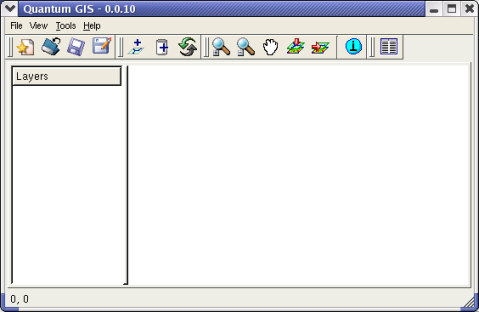
\includegraphics{./qgismain.png}
\end{figure}


Plugins are free to implement additional GUI elements or windows to
accomplish their task(s).


\subsection{Plugins}

QGIS will rely heavily on plugins to implement all major functions.
With a flexible plugin architecture, QGIS can be easily extended to
support additional features and capabilities. 


\subsubsection{Class Diagram}

The class diagram in Figure \ref{cap:Conceptual-Diagram-of} provides
a conceptual model of QGIS with regard to plugins.%
\begin{figure}[h]

\caption{\label{cap:Conceptual-Diagram-of}Conceptual Diagram of Plugin Architecture}
\smallskip{}


\includegraphics{./plugin.png}
\end{figure}



\subsubsection{Plugin Load Sequence}

The main application class uses QLibrary to load and resolve plugin
functions. In order for a plugin to be recognized, it must implement
the methods defined in the QgisPlugin abstract class and also return
a valid version string when queried by the main application. The sequence
of events when a plugin is loaded is:

\begin{enumerate}
\item QGIS attempts to load the plugin's shared library using QLibary::load().
\item If load succeeds, the classFactory method is resolved using QLibrary::resolve().
The classFactory method is declared as extern {}``C'' and is responsible
for creating an instance of the plugin and returning a pointer to
it.
\item If the classFactory method is resolved successfully, QGIS calls the
method, passing a pointer to the one and only instance of QgisInterface.
\item Once the plugin instance is created, the plugin can do any initialization
required, including adding menus and toolbars to the using the QgisInterface
pointer.
\end{enumerate}

\subsection{\label{sub:Data-Providers}Data Providers}

\begin{comment}
Data providers are a kind of plugin, but they're very different. So,
I put this in a separate section. However, it's still plugin-like.
So should it be rolled into the previous subsection?
\end{comment}
Data providers are a special kind of plug-in. qgis uses data providers
to implement geospatial data I/O for specific formats. The notion
is that support for additional geospatial formats can easily added
by merely creating a data provider plug-in that supports a given format.
Moreover it should be possible to have multiple support for the same
format; that is, have more than one data provider available to load
a given geospatial data type. Figure \ref{cap:DataProvider} depicts
the data provider class hierarchy.

%
\begin{figure}
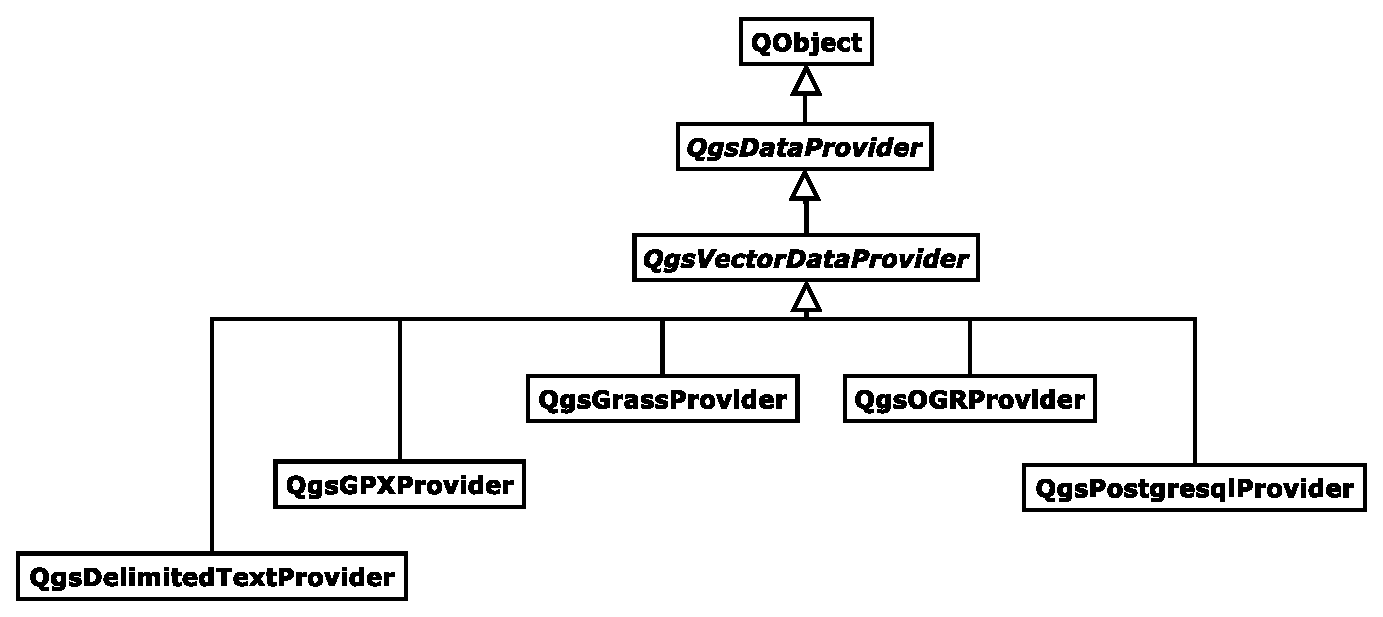
\includegraphics[%
  width=1.0\columnwidth]{dataprovider.eps}


\caption{\label{cap:DataProvider}Data provider class hierarchy}
\end{figure}


Note that currently there is no \texttt{QgsRasterDataProvider} sub-hierarchy,
though that will change in a subsequent design refactoring. Currently
\texttt{QgsRasterLayer} manages its own data I/O directly through
GDAL library calls.

The data provider plug-ins use a different loading method than for
the general qgis plug-ins. 

All data provider plug-in information is managed by the \texttt{QgsProviderRegistry}
Singleton object. When initially created it searches the plug-in path
for all data provider plug-ins. It does this by visiting each dynamic
object in the path (\texttt{.DLL} in Windows, and \texttt{.so} in
{*}nix environments); if the dynamic loader is able to resolve the
symbol \texttt{isProvider}, then the currently loaded dynamic object
is indeed a data provider. In that case, a \texttt{QgsProviderMetadata}
object is created which stores a provider name, description, and full
file name; this information is loaded from the dynamic object via
calls to its \texttt{providerKey()}, \texttt{description()} and \texttt{library()}
functions, respectively. The \texttt{QgsProviderRegistry} Singleton
keeps an internal associative container of these \texttt{QgsProviderMetadata}
objects keyed by the string returned from the providerKey() call.
The alternative to having these \texttt{QgsProviderMetata} objects
stored in this way would have been to load and keep \emph{all} the
data providers in memory during the application's lifetime regardless
if they would ultimately be used. Instead of wastefully keeping all
the data providers loaded, they are lazily loaded only when needed
via the mechanism that uses \texttt{QgsProviderMetadata} objects.
When a specific data provider is needed, the following steps are performed:

\begin{enumerate}
\item \texttt{QgsProviderRegistry::getProvider()} is invoked with a provider
key
\item The \texttt{QgsProviderMetadata} matching that key is retrieved
\item A \texttt{QLibrary::load()} call is made with the associated file
path found in the returned metadata \texttt{library()} call
\item The plug-in's \texttt{classFactory()} member is invoked with the data
source name as its argument
\item The created data provider returned from the \texttt{classFactory()}
invocation is then returned to the caller
\end{enumerate}
The data provider is owned by its associated layer, which is then
responsible for its destrction. (This will likely change in a subsequent
refactoring to address the problem of a data source having more than
one layer.)


\subsection{Layers}

As described \vpageref{des:Layer:-A-dataset} layer is a set of related
geospatial data and their associated attributes. Layers tend to contain
a particular type of data, such as hydrography, transportation, and
hypsography data. Layers therefore tend to be {}``thematic'' in
nature. There are two kinds of qgis layers that follow from their
representations -- vector and raster layers. Figure \ref{cap:maplayer}
shows the \texttt{QgsMapLayer} hierarchy that qgis uses to implement
vector and raster layers.

%
\begin{figure}
\includegraphics[%
  width=1.0\columnwidth]{maplayer.eps}


\caption{\label{cap:maplayer}QgsMapLayer Class Hierarchy}
\end{figure}


\begin{comment}
Add stuff to describe layer contents. This would start with general
common things found in QgsMapLayer followed by descriptions for each
of the subclasses. Try to emphasize the static attributes -- the dynamic
aspects on HOW they'll be used will be in subsequent chapters.

Need to talk about renderers.

And especially about coordinate transforms.
\end{comment}
Layers have a unique identification string and a separate string for
a base name. They also have a source string which can contain a file
name or URI. The base name is used to identify the layer in the legend.

The \texttt{QgsMapLayerRegistry} is the Singleton object that stores
all canonical layer instances. QgsMapLayerRegistry supports three
Qt signals. \texttt{layerWasAdded()} is raised when a new layer is
added to the registry. \texttt{layerWillBeRemoved()} is raised if
a layer is to be deleted. \texttt{removeAll()} is raised if all the
layers are to be cleared. The last is an optimization for clearing
all layers at once instead of raising a signal for each layer that's
removed when, say, clearing a project.


\section{Use Case Scenario Design}

In this section we describe the underlying design that supports the
various use case scenarios given in section \ref{sec:Use-Cases}.


\subsection{Load Data}

This use case, as described \vpageref{sub:Load-Data}, is of course
for when the user loads data into qgis. Though vector and raster layers
share many features, they are very different especially in how they
respectively load data.


\subsubsection{Vector Layer Loading}

A new \texttt{QgsVectorLayer} is created when \texttt{QgisApp::addLayer()},
\texttt{QgisApp::addDatabaseLayer()}, or \texttt{QgsProject::read()}
are invoked. The newly created \texttt{QgsVectorLayer} is given the
file path for the data source, the basename of that file path as its
name, and a data provider key used to find an appropriate data provider
from the data provider registry described in section \ref{sub:Data-Providers}.
The data provider key will be {}``ogr'' if for a file based format
since only the OGR data provider is the one currently supporting such.
If PostGIS support is enabled, the data provider key can be {}``postgres''
so the data provider registry can find the PostgreSQL/PostGIS data
provider. (Yes, but this only happens when addDatabaseLayer is invoked.
May need to further break this down or re-organize.)


\subsubsection{Raster Layer Loading}

Also triggered by QgisApp::addLayer() or QgsProject::read() a new
\texttt{QgsRasterLayer} is created.
\end{document}
